% \documentclass[hidelinks,12pt]{article}
\usepackage[left=0.25cm,top=1cm,right=0.25cm,bottom=1cm]{geometry}
%\usepackage[landscape]{geometry}
\textwidth = 20cm
\hoffset = -1cm
\usepackage[utf8]{inputenc}
\usepackage[spanish,es-tabla]{babel}
\usepackage[autostyle,spanish=mexican]{csquotes}
\usepackage[tbtags]{amsmath}
\usepackage{nccmath}
\usepackage{amsthm}
\usepackage{amssymb}
\usepackage{mathrsfs}
\usepackage{graphicx}
\usepackage{subfig}
\usepackage{standalone}
\usepackage[outdir=./Imagenes/]{epstopdf}
\usepackage{siunitx}
\usepackage{physics}
\usepackage{color}
\usepackage{float}
\usepackage{hyperref}
\usepackage{multicol}
%\usepackage{milista}
\usepackage{anyfontsize}
\usepackage{anysize}
%\usepackage{enumerate}
\usepackage[shortlabels]{enumitem}
\usepackage{capt-of}
\usepackage{bm}
\usepackage{relsize}
\usepackage{placeins}
\usepackage{empheq}
\usepackage{cancel}
\usepackage{wrapfig}
\usepackage[flushleft]{threeparttable}
\usepackage{makecell}
\usepackage{fancyhdr}
\usepackage{tikz}
\usepackage{bigints}
\usepackage{scalerel}
\usepackage{pgfplots}
\usepackage{pdflscape}
\pgfplotsset{compat=1.16}
\spanishdecimal{.}
\renewcommand{\baselinestretch}{1.5} 
\renewcommand\labelenumii{\theenumi.{\arabic{enumii}})}
\newcommand{\ptilde}[1]{\ensuremath{{#1}^{\prime}}}
\newcommand{\stilde}[1]{\ensuremath{{#1}^{\prime \prime}}}
\newcommand{\ttilde}[1]{\ensuremath{{#1}^{\prime \prime \prime}}}
\newcommand{\ntilde}[2]{\ensuremath{{#1}^{(#2)}}}

\newtheorem{defi}{{\it Definición}}[section]
\newtheorem{teo}{{\it Teorema}}[section]
\newtheorem{ejemplo}{{\it Ejemplo}}[section]
\newtheorem{propiedad}{{\it Propiedad}}[section]
\newtheorem{lema}{{\it Lema}}[section]
\newtheorem{cor}{Corolario}
\newtheorem{ejer}{Ejercicio}[section]

\newlist{milista}{enumerate}{2}
\setlist[milista,1]{label=\arabic*)}
\setlist[milista,2]{label=\arabic{milistai}.\arabic*)}
\newlength{\depthofsumsign}
\setlength{\depthofsumsign}{\depthof{$\sum$}}
\newcommand{\nsum}[1][1.4]{% only for \displaystyle
    \mathop{%
        \raisebox
            {-#1\depthofsumsign+1\depthofsumsign}
            {\scalebox
                {#1}
                {$\displaystyle\sum$}%
            }
    }
}
\def\scaleint#1{\vcenter{\hbox{\scaleto[3ex]{\displaystyle\int}{#1}}}}
\def\bs{\mkern-12mu}


% \title{Transformada de Fourier \\ \Large{Ejercicios}} \vspace{-3ex}
% \author{M. en C. Gustavo Contreras Mayén}
% \date{ }
% \newcommand{\Cancel}[2][black]{{\color{#1}\cancel{\color{black}#2}}}
% \begin{document}
% \vspace{-4cm}
% \maketitle
% \fontsize{14}{14}\selectfont
% \tableofcontents
% \newpage
\documentclass[12pt]{beamer}
\usepackage{../Estilos/BeamerMAF}
\usepackage[absolute, overlay]{textpos}
\usepackage{../Estilos/ColoresLatex}
%Sección para el tema de beamer, con el theme, usercolortheme y sección de footers
\usetheme{Antibes}
\usecolortheme{beaver}
%\useoutertheme{default}
\setbeamercovered{invisible}
% or whatever (possibly just delete it)
\setbeamertemplate{section in toc}[sections numbered]
\setbeamertemplate{subsection in toc}[subsections numbered]
\setbeamertemplate{subsection in toc}{\leavevmode\leftskip=3.2em\rlap{\hskip-2em\inserttocsectionnumber.\inserttocsubsectionnumber}\inserttocsubsection\par}
\setbeamercolor{section in toc}{fg=blue}
\setbeamercolor{subsection in toc}{fg=blue}
%\setbeamercolor{frametitle}{fg=blue}
\setbeamertemplate{caption}[numbered]

\setbeamertemplate{footline}
\beamertemplatenavigationsymbolsempty
\setbeamertemplate{headline}{}


\makeatletter
\setbeamercolor{secºtion in foot}{bg=gray!30, fg=black!90!orange}
\setbeamercolor{subsection in foot}{bg=blue!30!yellow, fg=red}
\setbeamercolor{date in foot}{bg=black, fg=white}
\setbeamertemplate{footline}
{
  \leavevmode%
  \hbox{%
  \begin{beamercolorbox}[wd=.333333\paperwidth,ht=2.25ex,dp=1ex,center]{section in foot}%
    \usebeamerfont{section in foot} \insertsection
  \end{beamercolorbox}%
  \begin{beamercolorbox}[wd=.333333\paperwidth,ht=2.25ex,dp=1ex,center]{subsection in foot}%
    \usebeamerfont{subsection in foot}  \insertsubsection
  \end{beamercolorbox}%
  \begin{beamercolorbox}[wd=.333333\paperwidth,ht=2.25ex,dp=1ex,right]{date in head/foot}%
    \usebeamerfont{date in head/foot} \insertshortdate{} \hspace*{2em}
    \insertframenumber{} / \inserttotalframenumber \hspace*{2ex} 
  \end{beamercolorbox}}%
  \vskip0pt%
}







\setbeamercolor{section in foot}{bg=amethyst, fg=white}
\setbeamercolor{subsection in foot}{bg=almond, fg=black}

\makeatletter
\setbeamertemplate{footline}
{
\leavevmode%
\hbox{%
\begin{beamercolorbox}[wd=.333333\paperwidth,ht=2.25ex,dp=1ex,center]{section in foot}%
  \usebeamerfont{section in foot} \insertsection
\end{beamercolorbox}%
\begin{beamercolorbox}[wd=.333333\paperwidth,ht=2.25ex,dp=1ex,center]{subsection in foot}%
  \usebeamerfont{subsection in foot}  \insertsubsection
\end{beamercolorbox}%
\begin{beamercolorbox}[wd=.333333\paperwidth,ht=2.25ex,dp=1ex,right]{date in head/foot}%
  \usebeamerfont{date in head/foot} \insertshortdate{} \hspace*{1.5em}
  \insertframenumber{} / \inserttotalframenumber \hspace*{2ex} 
\end{beamercolorbox}}%
\vskip0pt%
}
\makeatother
\usefonttheme{serif}
\setbeamercolor{frametitle}{bg=champagne}
\resetcounteronoverlays{saveenumi}

\date{}

\title{\large{Tema 6 - Transformada de Laplace}}
\subtitle{Matemáticas Avanzadas de la Física}
\author{M. en C. Gustavo Contreras Mayén}

\begin{document}
\maketitle
\fontsize{14}{14}\selectfont
\spanishdecimal{.}

\section*{Contenido}
\frame[allowframebreaks]{\frametitle{Temas a revisar} \tableofcontents[currentsection, hideallsubsections]}


\section{La Transformada de Fourier}
\frame{\tableofcontents[currentsection, hideothersubsections]}
\subsection{Áreas de aplicación}

\begin{frame}
\frametitle{Dónde usar la TF}
Las aplicaciones de la Transformada de Fourier (TF) son muy extensas, ya que abarcan diversas ramas de la física matemática.
\end{frame}
\begin{frame}
\frametitle{Dónde usar la TF}
\setbeamercolor{item projected}{bg=bananayellow,fg=ao}
\setbeamertemplate{enumerate items}{%
\usebeamercolor[bg]{item projected}%
\raisebox{1.5pt}{\colorbox{bg}{\color{fg}\footnotesize\insertenumlabel}}%
}
\begin{enumerate}[<+->]
\item Teoría de números.
\item Geometría.
\item Óptica.
\item Mecánica cuántica.
\item Medicina.
\seti
\end{enumerate}    
\end{frame}
\begin{frame}
\frametitle{Dónde usar la TF}
\setbeamercolor{item projected}{bg=bananayellow,fg=ao}
\setbeamertemplate{enumerate items}{%
\usebeamercolor[bg]{item projected}%
\raisebox{1.5pt}{\colorbox{bg}{\color{fg}\footnotesize\insertenumlabel}}%
}
\begin{enumerate}[<+->]
\conti
\item Comunicaciones.
\item Ingeniería biomédica.
\item Procesamiento de señales de audio.
\item Procesamiento de imágenes.
\end{enumerate}    
\end{frame}
\begin{frame}
\frametitle{Dónde usar la TF}
La TF también se utiliza para:
\pause
\setbeamercolor{item projected}{bg=white,fg=black}
\setbeamertemplate{enumerate items}{%
\usebeamercolor[bg]{item projected}%
\raisebox{1.5pt}{\colorbox{bg}{\color{fg}\footnotesize\insertenumlabel}}%
}
\begin{enumerate}[<+->]
\item Analizar contenido de frecuencia de las señales.
\item Determinar como cambia la amplitud y las fases de las señales sinusoidales cuando éstas pasan a través de un sistema lineal e invariante en el tiempo.
\seti
\end{enumerate}    
\end{frame}
\begin{frame}
\frametitle{Dónde usar la TF}
\setbeamercolor{item projected}{bg=white,fg=black}
\setbeamertemplate{enumerate items}{%
\usebeamercolor[bg]{item projected}%
\raisebox{1.5pt}{\colorbox{bg}{\color{fg}\footnotesize\insertenumlabel}}%
}
\begin{enumerate}[<+->]
\conti
\item Generar formas de onda de corriente o tensión eléctrica por medio de la superposición de señales senoidales generadas por osciladores electrónicos de amplitud variable cuyas frecuencias ya están determinadas.
\item Analizar el comportamiento armónico de una señal.
\end{enumerate}
\end{frame}

\subsection{Ejemplos concretos}

\begin{frame}
\frametitle{Electromagnetismo}
En el campo del electromagnetismo y de microondas, la Transformada de Fourier está relacionada con:
\pause
\begin{itemize}
\item El cálculo del campo cercano transitorio que es irradiado por dispositivos electrónicos.
\item El análisis de fenómenos ópticos en microondas.
\item El cálculo del campo electromagnético de rayos, la formación de haz y la radiación de microondas solares.
\end{itemize}
\end{frame}
\begin{frame}
\frametitle{Medicina}    
En Medicina, el análisis de la TF está relacionado con:
\pause
\begin{itemize}
\item El análisis espectral del comportamiento global de los cromosomas.
\item El análisis espectral de la variabilidad de la frecuencia cardíaca.
\item El procesamiento de imágenes generadas por econogramas, resonancias magnéticas y tomografía axial.
\end{itemize}
\end{frame}
\begin{frame}
\frametitle{Comunicaciones}    
En el área de comunicaciones se usa para:
\pause
\begin{itemize}
\item Analizar la frecuencia de señales.
\item Diseñar los sistemas de transmisión de señales para transmitir información.
\item Diseñar supresores y canceladores de ecos en líneas telefónicas.
\end{itemize}
\end{frame}
\begin{frame}
\frametitle{Mecánica}    
En el campo de la ingeniería mecánica:
\pause
\begin{itemize}
\item  Se utiliza para balancear rotores y eliminar la vibración que se genera cuando no están balanceados.
\item Estudiar los problemas relacionados con vibraciones mecánicas en los motores, generadores y equipos rotatorios en general.
\end{itemize}
\end{frame}
\begin{frame}
\frametitle{Análisis señales de audio}    
En el procesamiento de señales de audio:
\pause
\begin{itemize}
\item Se usa para compactar las señales de audio (formatos MP3 y MP4).
\item Producir efectos de sonido, diseñar sintetizadores de audio y ecualizadores.
\end{itemize}
\end{frame}
\begin{frame}
\frametitle{Procesamiento de imágenes}    
En un campo extendido del procesamiento de imágenes:
\pause
\begin{itemize}
\item La TF se utiliza para filtrar imágenes, extraer características de interés.
\item Realizar transformaciones de imágenes y compactar imágenes.
\end{itemize}
Algo de lo que podemos hacer con la TF de una imagen es eliminar algunos componentes.
\end{frame}
\begin{frame}
\frametitle{Manejando imágenes}    
Si eliminamos las frecuencias bajas, menores de cierto valor $\omega_{f}$, \pause se le llama \textocolor{armygreen}{filtro de paso alto}.
\\
\bigskip
\pause
Una gran cantidad de ruido de fondo se produce a bajas frecuencias, por lo que un filtro de paso alto puede limpiar una señal.
\end{frame}
\begin{frame}
\frametitle{Manejando imágenes}
Si descartamos las frecuencias altas, se llama \textocolor{cobalt}{filtro de paso bajo}.
\\
\bigskip
\pause
Se puede usar un filtro de paso bajo para suavizar los datos (como una foto digital), ya que arroja ruido de alta frecuencia. \pause Un filtro que corta las frecuencias altas y bajas se llama \textocolor{blue}{filtro de paso de banda}.
\end{frame}

\subsection{Manejando una imagen}

\begin{frame}
\frametitle{Software para el manejo de una imagen}
En el software para manejo de imágenes como Photshop, GIMP, Picasa, etc. se cuenta con un conjunto de filtros que modifican la apariencia de una imagen, \pause ya sea con la finalidad de corregir detalles o mejorar la misma.
\end{frame}
\begin{frame}
\frametitle{Software para el manejo de una imagen}
Básicamente se están utilizando TF, \pause pero no se le llaman de esta manera, sino que le dan otros nombres comercialmente más atractivos dentro del software.
\end{frame}
\begin{frame}
\frametitle{Ejemplo de manejo con imágenes}
A continuación veremos un ejemplo de la aplicación de un filtro pasa altos en una imagen:
\pause
\setbeamercolor{item projected}{bg=blue,fg=white}
\setbeamertemplate{enumerate items}{%
\usebeamercolor[bg]{item projected}%
\raisebox{1.5pt}{\colorbox{bg}{\color{fg}\footnotesize\insertenumlabel}}%
}
\begin{enumerate}[<+->]
\item A la izquierda tenemos la imagen original.
\item Mientras que a la derecha la imagen resultante luego de ocupar el filtro pasa altos.
\end{enumerate}
\end{frame}
\begin{frame}[plain]
\begin{figure}[H]
    \centering
    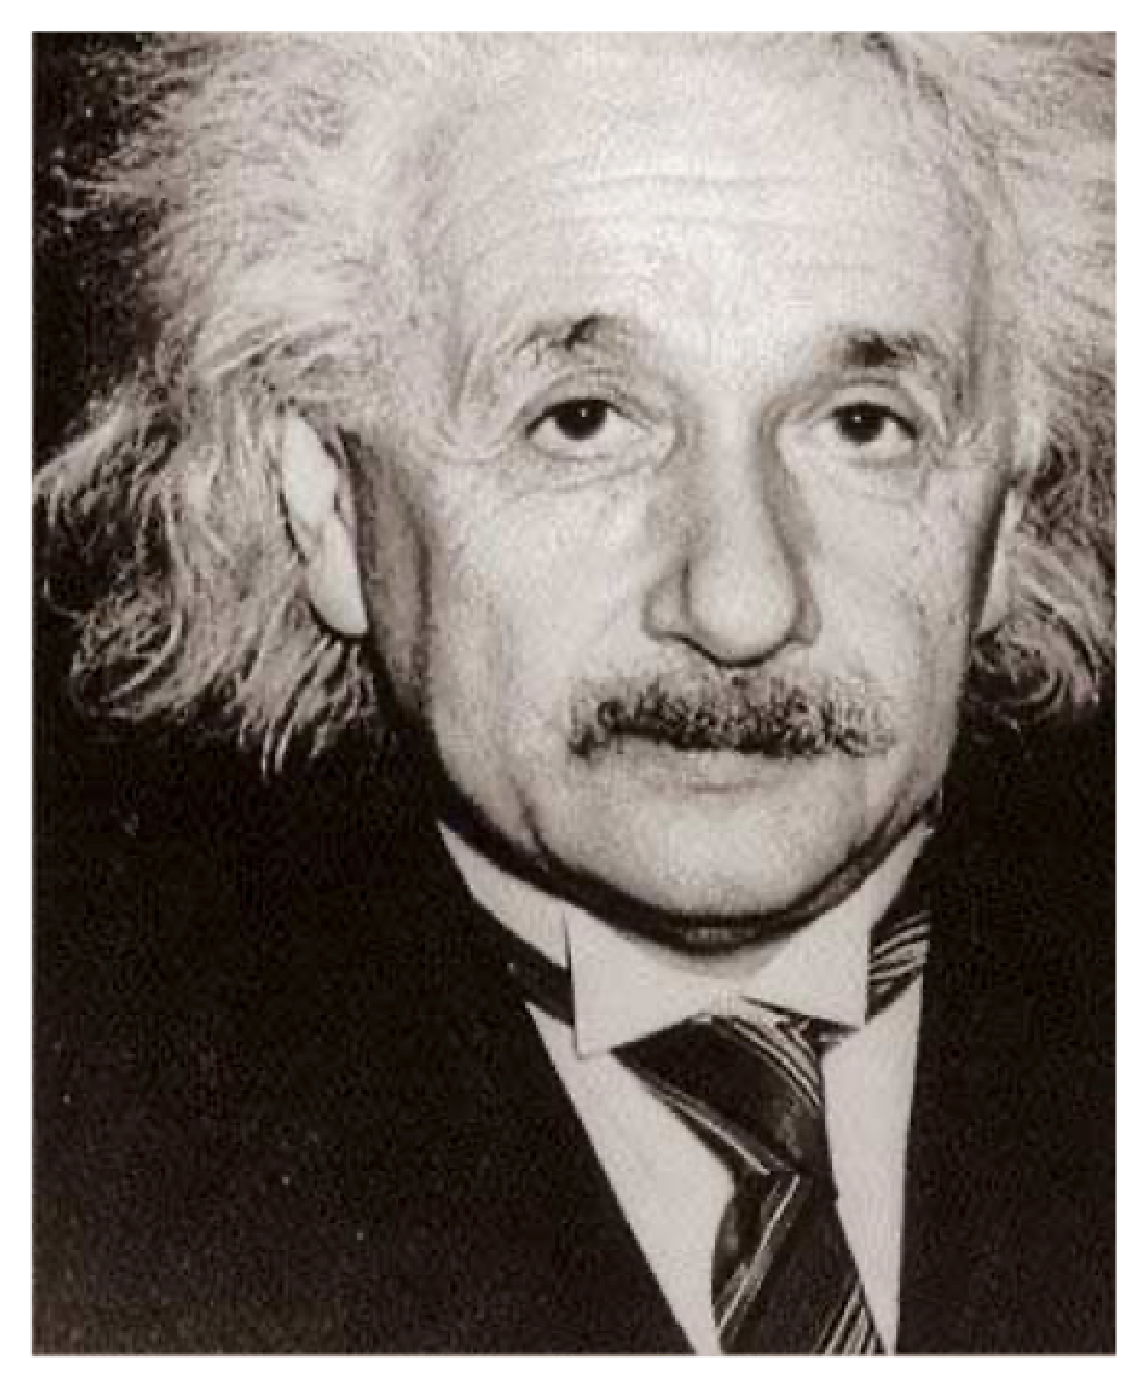
\includegraphics[scale=0.25]{Imagenes/Einstein_01.eps}
    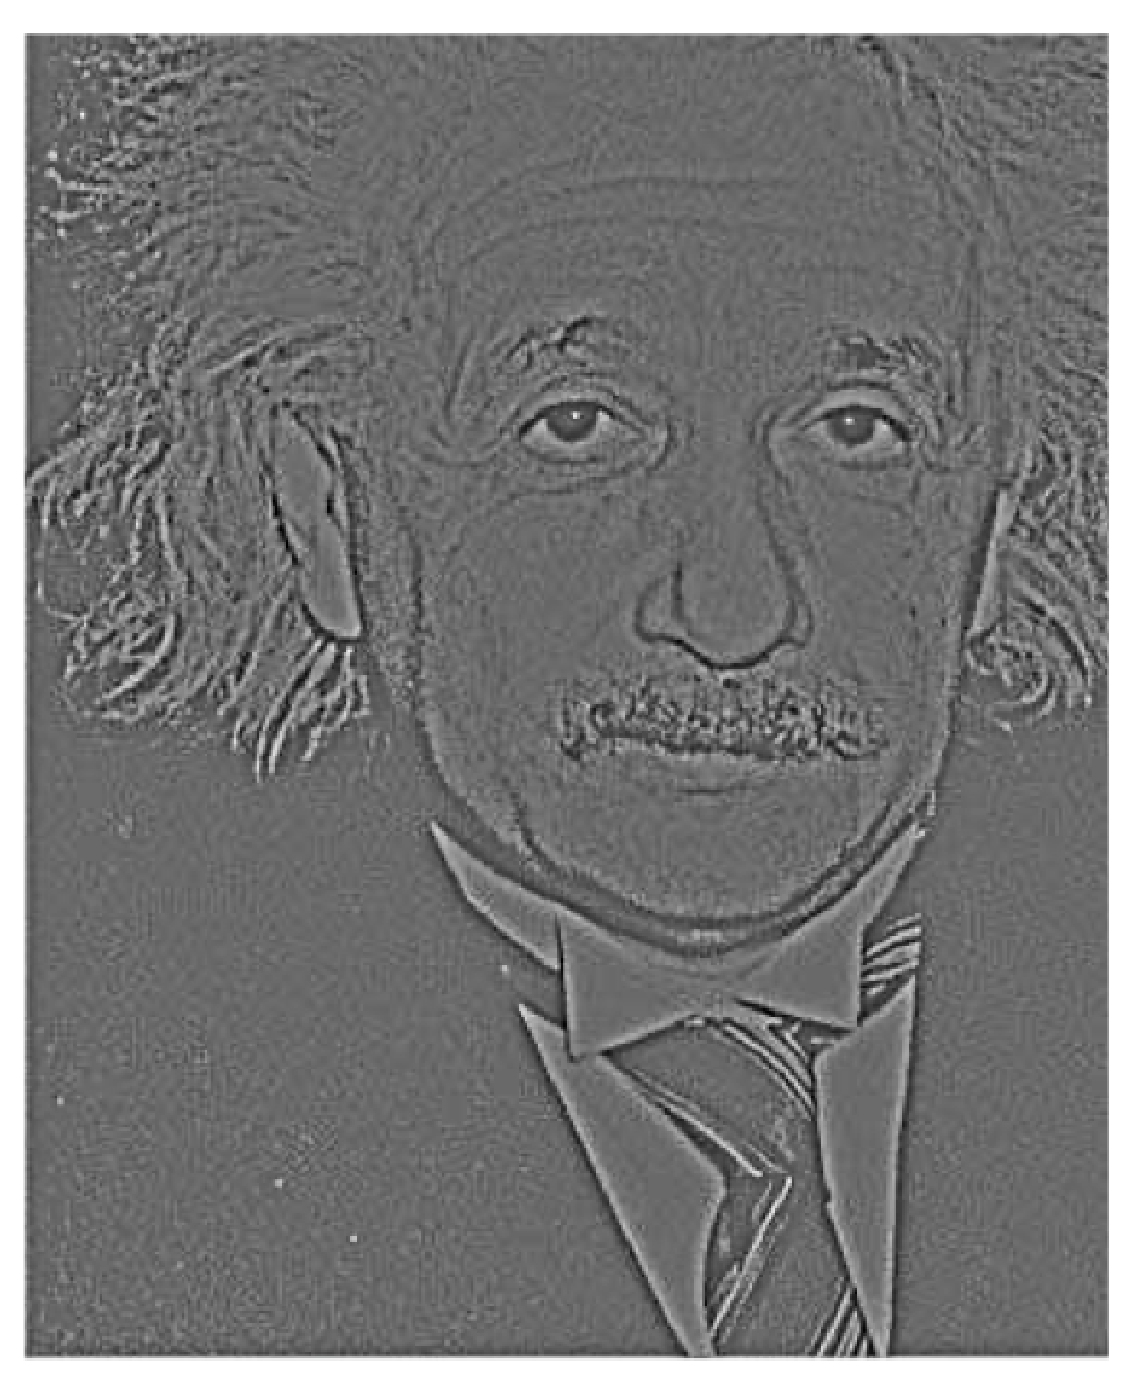
\includegraphics[scale=0.25]{Imagenes/Einstein_02.eps}
\end{figure}
\end{frame}
\begin{frame}
\frametitle{Ejemplo de manejo con imágenes}
En el siguiente ejemplo se presenta la aplicación de un filtro pasa bajos sobre otra imagen, \pause  nuevamente a la izquierda se presenta la imagen original y a la derecha, \pause la imagen resultante luego de ocupar el filtro.
\end{frame}
\begin{frame}[plain]
\begin{figure}
    \centering
    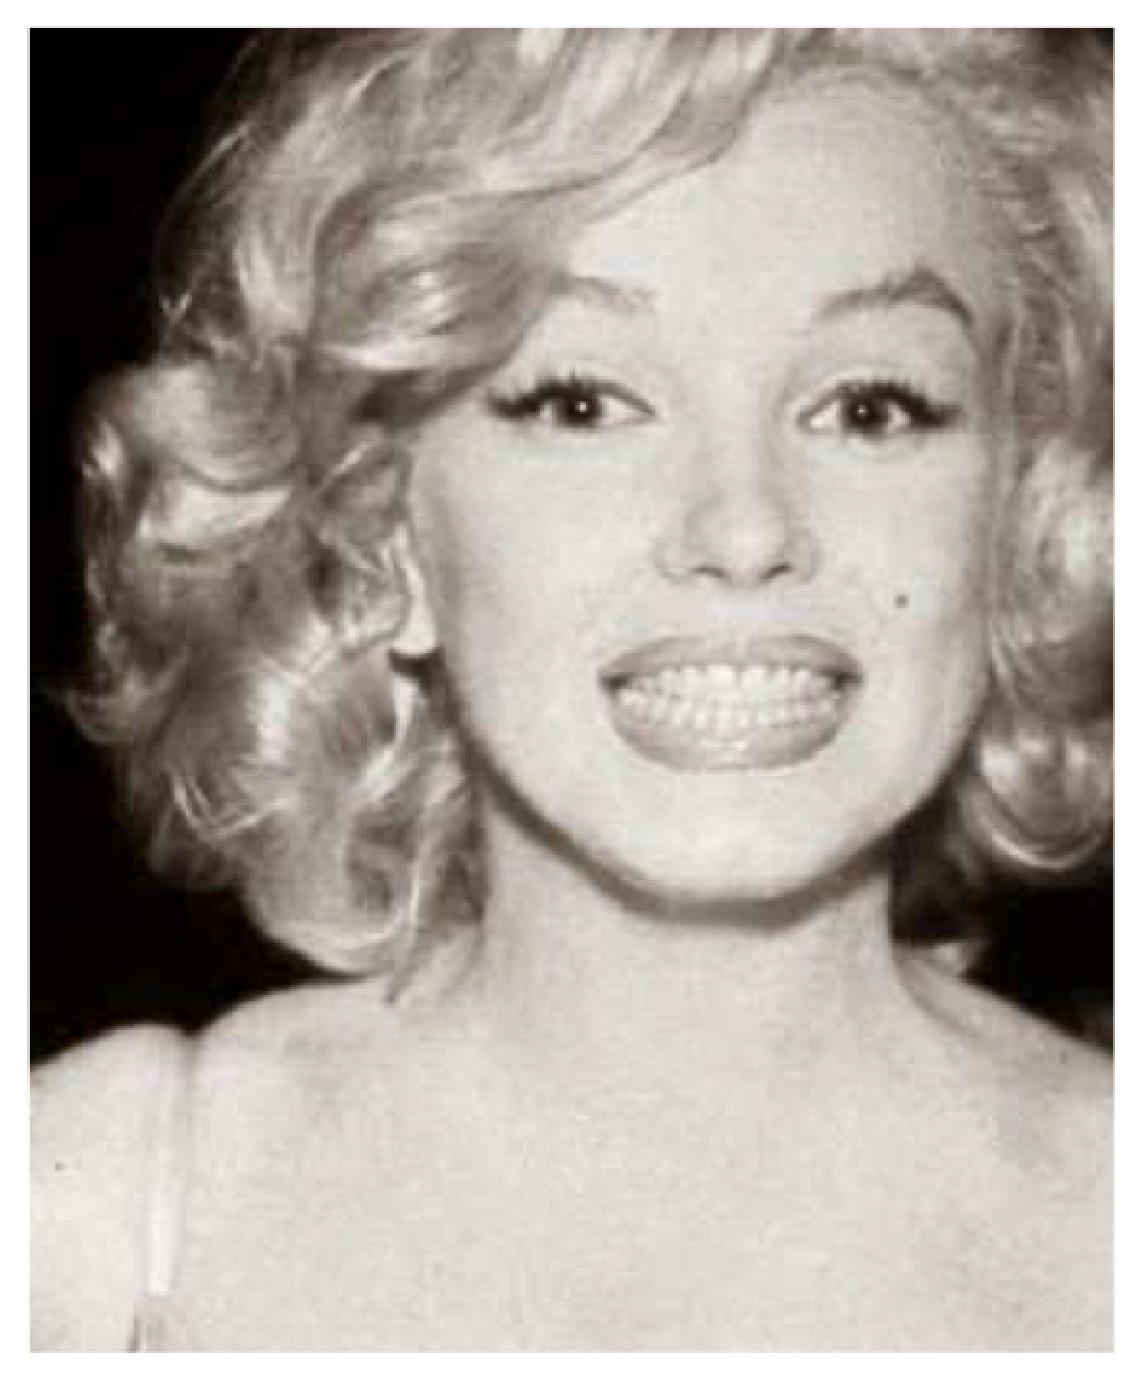
\includegraphics[scale=0.25]{Imagenes/Marylin_01.eps}
    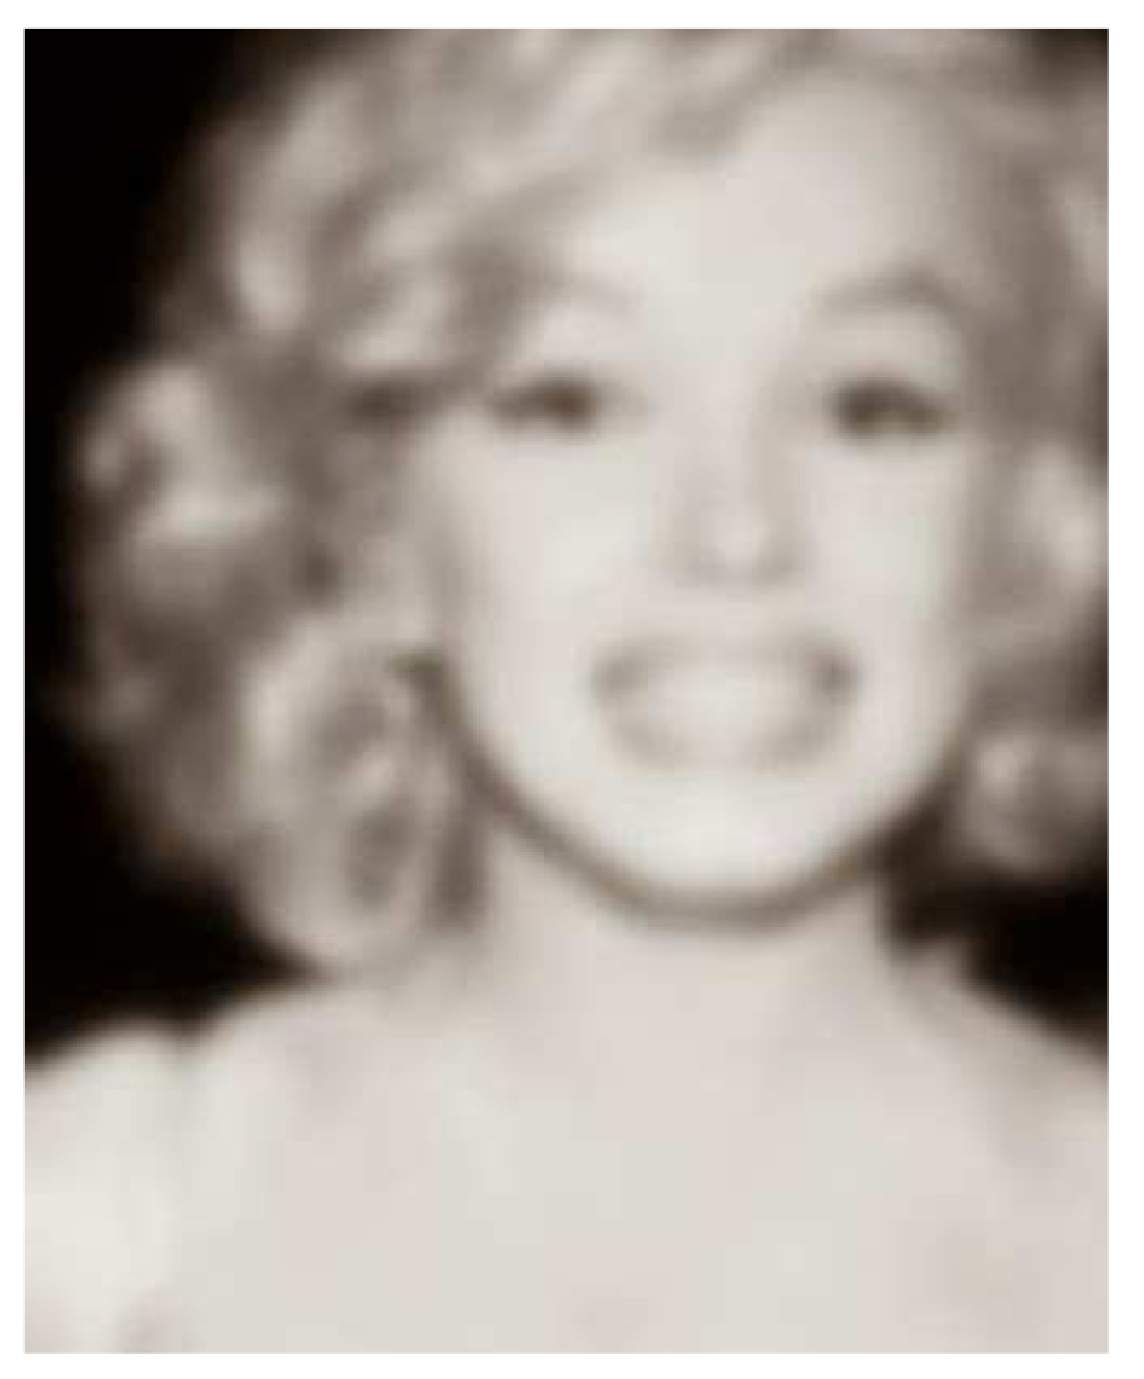
\includegraphics[scale=0.25]{Imagenes/Marylin_02.eps}
\end{figure}
\end{frame}
\begin{frame}
\frametitle{Ejemplo de manejo con imágenes}
Veamos que el resultado obtenido \textocolor{red}{desenfoca} la imagen original.
\end{frame}
\begin{frame}
\frametitle{Ejemplo de manejo con imágenes}
Si combinamos los filtros pasa alto en la imagen de Einstein y el filtro pasa bajo en la imagen de Marylin, obtenemos:
\end{frame}
\begin{frame}[plain]
\begin{figure}[H]
    \centering
    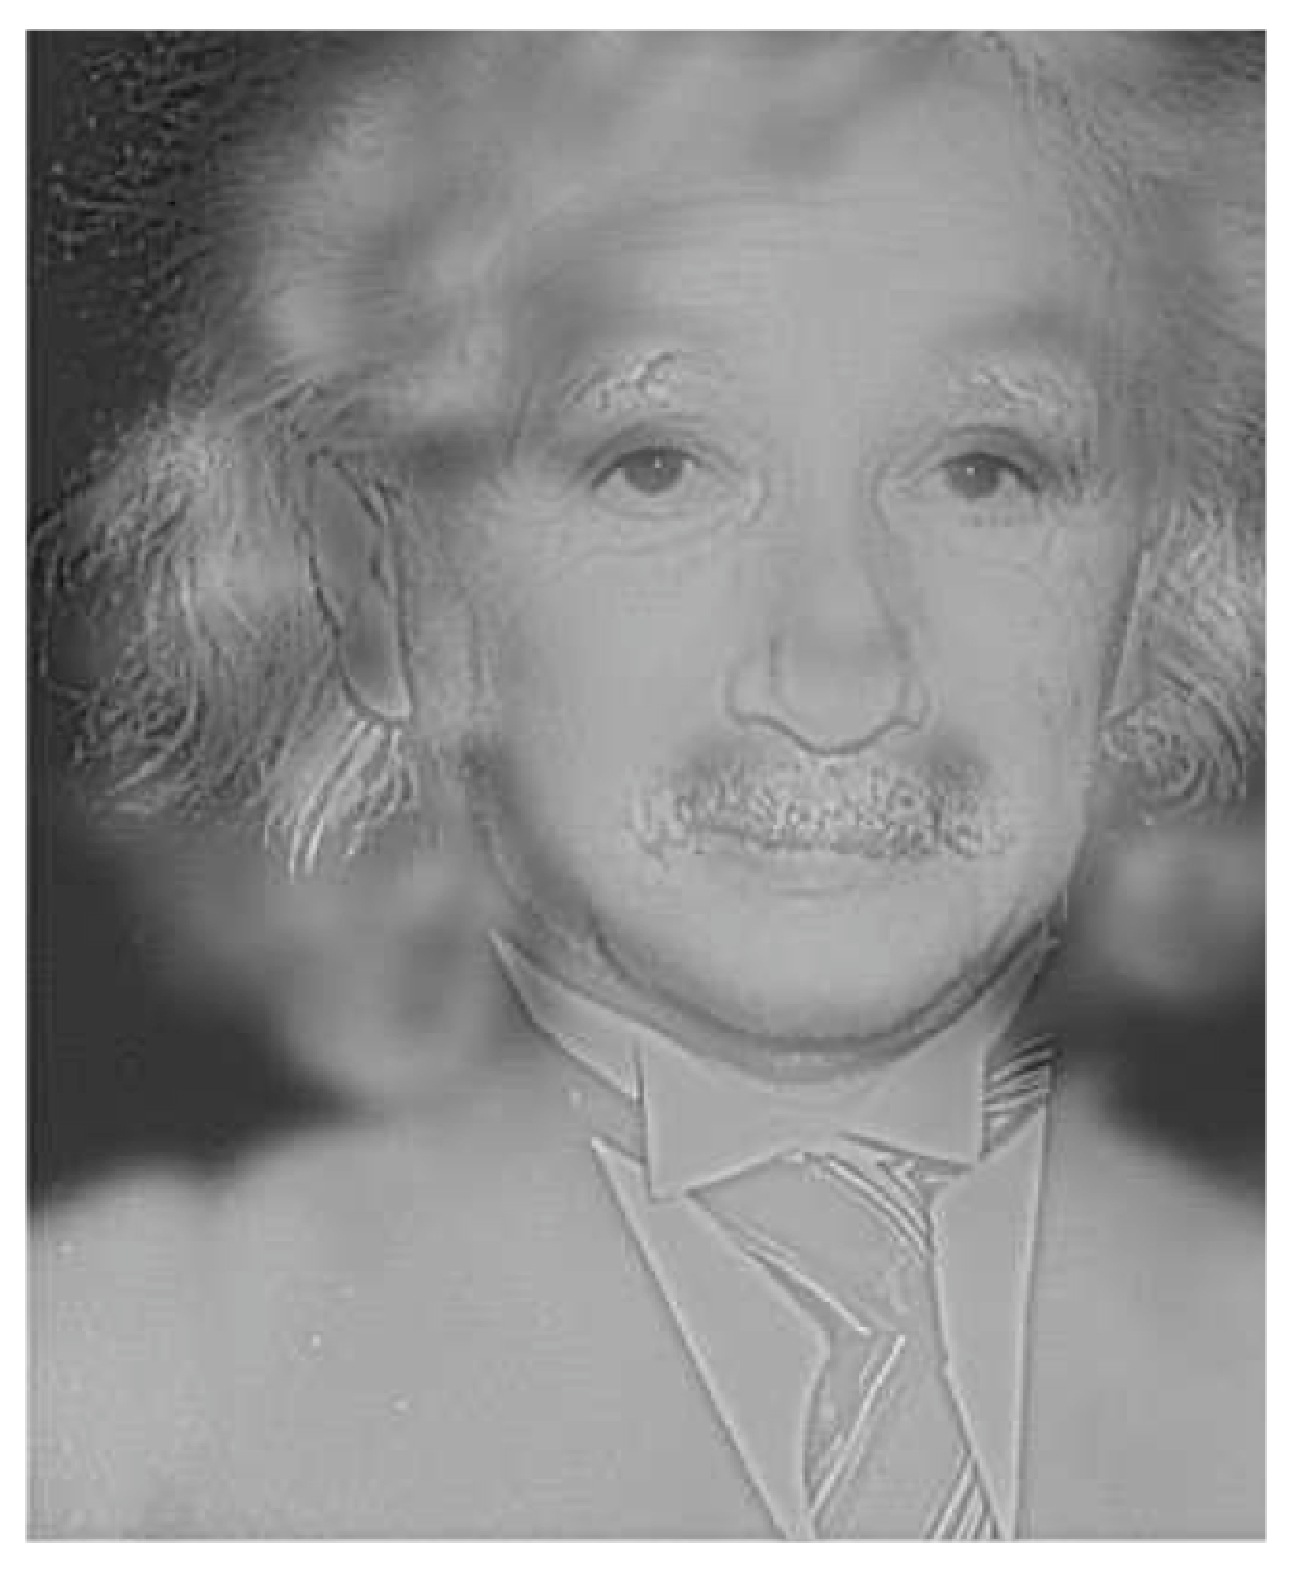
\includegraphics[scale=0.3]{Imagenes/Einstein_Marylin_AB_01.eps}
    % \caption{Filtro pasa alto Einstein + pasa bajo Marylin}
    \label{fig:figuraEpa_Mpb}
\end{figure}
\end{frame}
\begin{frame}
\frametitle{Ejemplo de manejo con imágenes}
Notamos una superposición de las dos imágenes, \pause curiosamente si nos acercamos a la imagen, nuestro cerebro procesa la información que recibe y perfila a uno de los dos personajes, \pause mientras que si nos alejamos de la imagen, reconocemos al otro personaje.
\end{frame}
\begin{frame}
\frametitle{Ejemplo de manejo con imágenes}
Hacemos el cambio de filtros: \pause en la imagen de Einstein se ocupa el filtro pasa bajo y en la imagen de Marylin, se ocupó el filtro pasa altos:
\end{frame}
\begin{frame}[plain]
\begin{figure}[H]
    \centering
    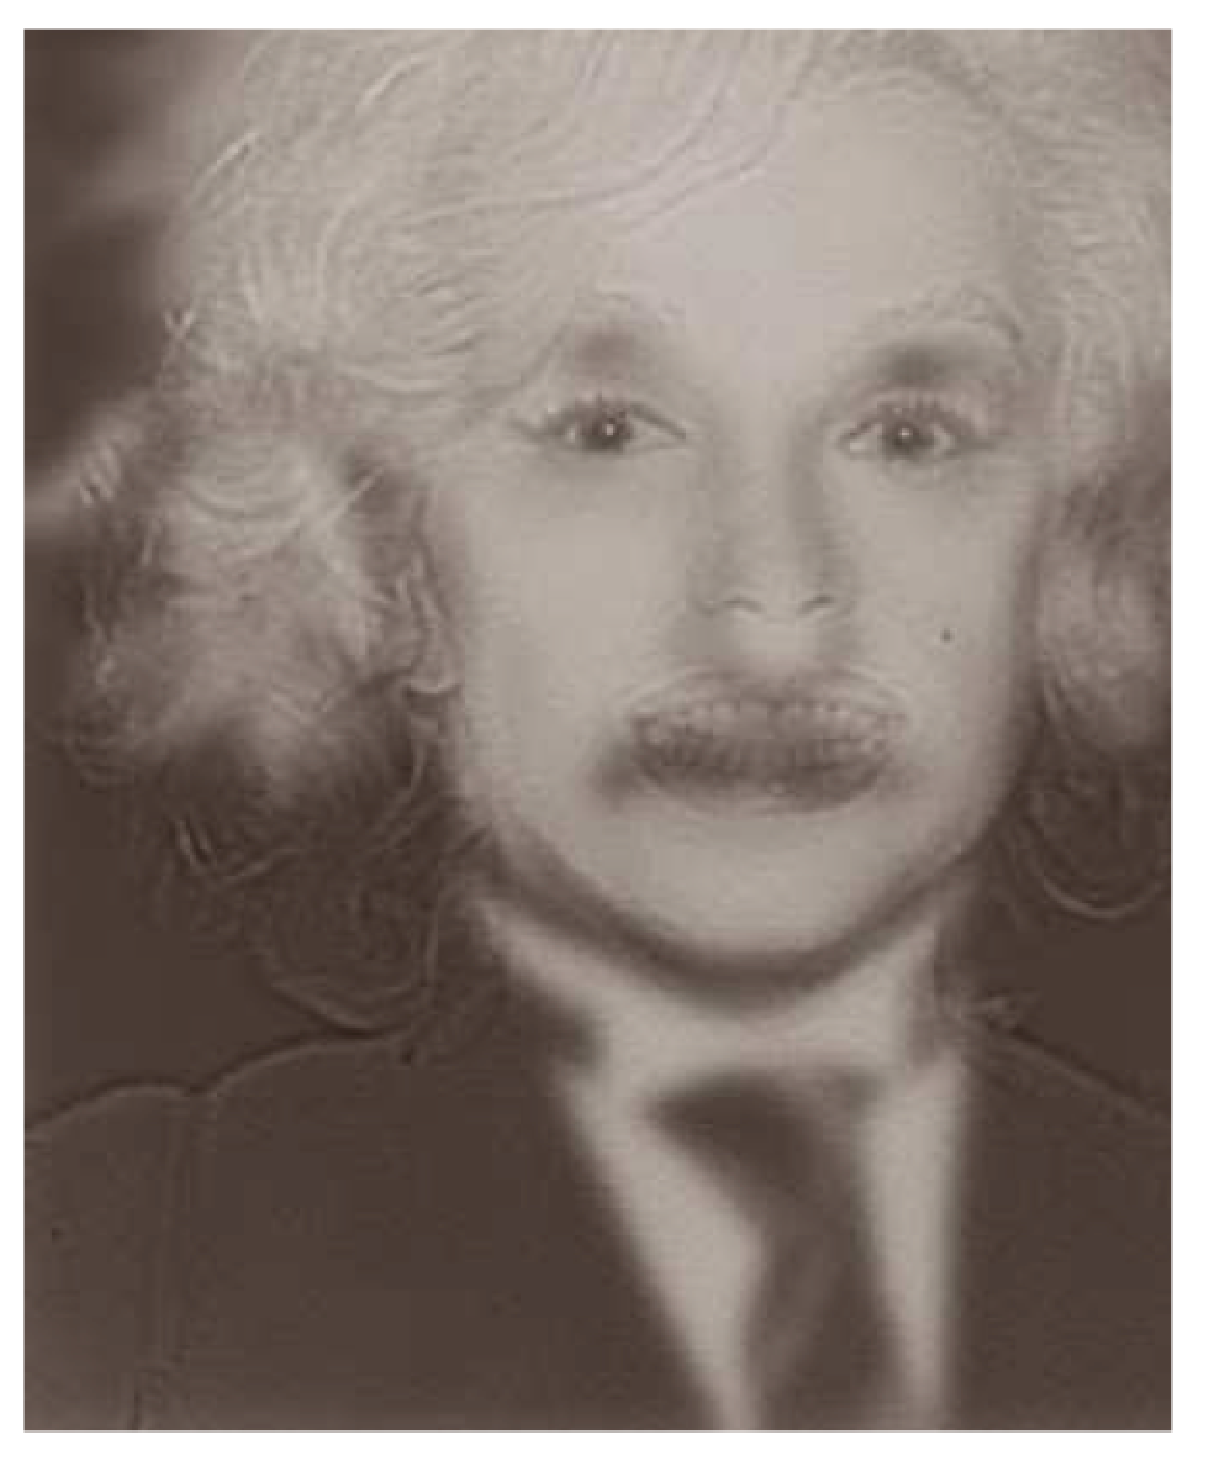
\includegraphics[scale=0.3]{Imagenes/Einstein_Marylin_BA_01.eps}
    % \caption{Filtro pasa bajo Einstein + pasa alto Marylin}
\end{figure}
\end{frame}
\begin{frame}
\frametitle{Ejemplo de manejo con imágenes}
¿Será que al invertir los filtros en las imágenes, ahora el personaje que se reconoce cuando nos acercamos es el contrario que en el caso de la imagen de la figura (\ref{fig:figuraEpa_Mpb})?
\end{frame}

\section{Transformada de Laplace}
\frame{\tableofcontents[currentsection, hideothersubsections]}
\subsection{Resonancia y factores cuadráticos}

\begin{frame}
\frametitle{Problema en particular}
Las siguientes dos transformadas inversas de Laplace son útiles para invertir fracciones parciales al caso de factores cuadráticos repetidos:
\pause
\begin{align}
&L^{-1} \left\{ \dfrac{1}{(s^{2} + k^{2})} \right\} = \dfrac{1}{ k} \, \sin k \, t \label{eq:ecuacion_07_03_16} \\[0.5em]
&L^{-1} \left\{ \dfrac{1}{(s^{2} + k^{2})^{2}} \right\} = \dfrac{1}{2 \, k^{3}} \, (\sin k \, t - k \, t \, \cos k \, t) \label{eq:ecuacion_07_03_17}
\end{align}
\end{frame}
\begin{frame}
\frametitle{Factores cuadráticos}
Debido a la presencia de los términos $t \, \sin k \, t$ y $t \, \cos k \, t$ en las ecs. (\ref{eq:ecuacion_07_03_16}) y (\ref{eq:ecuacion_07_03_17}), \pause un factor cuadrático repetido comúnmente indica la presencia del fenómeno de resonancia en un sistema mecánico no amortiguado o en un sistema eléctrico.
\end{frame}

\subsection{Oscilador sin fricción}

\begin{frame}
\frametitle{Enunciado del problema}
Resuelve el siguiente problema con valores iniciales:
\pause
\begin{align*}
\stilde{x} + \omega_{0}^{2} \, x = F_{0} \, \sin \omega \, t, \hspace{1cm} x(0) = \ptilde{x} (0) = 0
\end{align*}
que determinan las oscilaciones forzadas no amortiguadas de una masa sujeta a un resorte.
\end{frame}
\begin{frame}
\frametitle{Solución al problema}
Aplicando la TL a la ED, se obtiene la ecuación:
\pause
\begin{align*}
s^{2} \, X(s) + \omega^{2} \, X(s) = \dfrac{F_{0} \, \omega}{s^{2} + \omega^{2}}
\end{align*}
Recordemos la notación $X(s)$, representa la transformada de Laplace de la función $x(t)$.
\end{frame}
\begin{frame}
\frametitle{solución problema}    
Por lo que al despejar $X(s)$, tenemos que:
\pause
\begin{align*}
X(s) = \dfrac{F_{0} \, \omega}{(s^{2} + \omega^{2})(s^{2} + \omega_{0}^{2})}
\end{align*}
\end{frame}
\begin{frame}
\frametitle{solución problema}    
Por lo que habrá que revisar los dos casos:
\pause
\setbeamercolor{item projected}{bg=black,fg=white}
\setbeamertemplate{enumerate items}{%
\usebeamercolor[bg]{item projected}%
\raisebox{1.5pt}{\colorbox{bg}{\color{fg}\footnotesize\insertenumlabel}}%
}
\begin{enumerate}[<+->]
\item $\omega \neq \omega_{0}$.
\item $\omega = \omega_{0}$.
\end{enumerate}
\end{frame}

\subsection*{Caso 1}

\begin{frame}
\frametitle{Revisando el caso 1}
Si $\omega \neq \omega_{0}$, se encuentra que:
\pause
\begin{align*}
X(s) = \dfrac{F_{0} \, \omega}{\omega^{2} - \omega_{0}^{2}} \, \left( \dfrac{1}{s^{2}+ \omega_{0}^{2}} - \dfrac{1}{s^{2} + \omega^{2}} \right)
\end{align*}
\end{frame}
\begin{frame}
\frametitle{Revisando el caso 1}
De esta manera al aplicar la TLI, ec. (\ref{eq:ecuacion_07_03_16}), se concluye que la solución es:
\pause
\begin{align*}
x(t) = \dfrac{F_{0} \, \omega}{\omega^{2} - \omega_{0}^{2}} \left( \dfrac{1}{\omega_{0}} \sin \omega_{0} \, t - \dfrac{1}{\omega} \, \sin \omega \, t \right)
\end{align*}
\end{frame}

\subsection*{Caso 2}

\begin{frame}
\frametitle{Revisando el caso 2}
Pero si $\omega = \omega_{0}$, se tiene que:
\pause
\begin{align*}
X(s) = \dfrac{F_{0} \, \omega_{0}}{(s^{2} + \omega^{2})^{2}}
\end{align*}
\end{frame}
\begin{frame}
\frametitle{Revisando el caso 2}    
Aplicando la TLI, la ec. (\ref{eq:ecuacion_07_03_17}) obtenemos la solución de resonancia:
\pause
\begin{align}
x(t) = \dfrac{F_{0}}{2 \, \omega_{0}^{2}} \, (\sin \omega_{0} \, t - \omega_{0} \, t \, \cos \omega_{0} \, t )
\label{eq:ecuacion_07_03_18}
\end{align}
\end{frame}
\begin{frame}
\frametitle{Revisando el caso 2}
Proporcionando los valores $F_{0} = 1$ y $\omega = 0.5$ y graficando la solución, se tiene la siguiente figura, en donde podemos ver la solución de resonancia y las curvas envolventes.
\end{frame}
\begin{frame}[plain]
\begin{figure}[H]
    \centering
    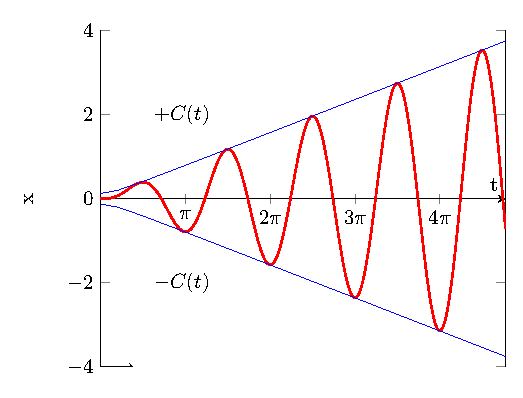
\includegraphics[scale=1]{Imagenes/sist_masa_resorte_resonancia_plot_01.eps}
    % \caption{La solución de resonancia junto con sus curvas envolventes.}
    \label{fig_figura_07_03_04}
\end{figure}
\end{frame}
\begin{frame}
\frametitle{De la solución}
La curva solución definida por la ec. (\ref{eq:ecuacion_07_03_18}) oscila una y otra vez entre dos \enquote{rectas envolventes}: $x = \pm \, C(t)$ (como vemos en la figura anterior) , que se obtienen al escribir la ec. (\ref{eq:ecuacion_07_03_18}) en la forma:
\pause
\begin{align*}
x(t) =  A(t) \, \cos \omega_{0} \, t +  B(t) \, \sin \omega_{0 \, t}
\end{align*}
\end{frame}
\begin{frame}
\frametitle{De la solución}
Definiendo entonces la usual \textocolor{bole}{amplitud}:
\pause
\begin{align*}
C = \sqrt{A^{2} +  B^{2}}
\end{align*}
\pause
En este caso se encuentra que:
\pause
\begin{align*}
C(t) = \dfrac{F_{0}}{2 \, \omega_{0}^{2}} \, \sqrt{\omega_{0}^{2} \, t^{2} + 1}
\end{align*}
\end{frame}

\subsection{Oscilador amortiguado}

\begin{frame}
\frametitle{Problema a resolver}
Con un sistema masa resorte amortiguador, considera los valores de $m = 1$, $k = 9.04$, $c= 0.4$ y $F(t) =  6 \, \exp(-t/5) \, \cos 3 \, t$.
\\
\bigskip
\pause
Con las condiciones iniciales:
\pause
\begin{align*}
x(0) = \ptilde{x}(0) = 0
\end{align*}
\end{frame}
\begin{frame}
\frametitle{Problema a resolver}    
Puntos a resolver:
\pause
\setbeamercolor{item projected}{bg=bananayellow,fg=red}
\setbeamertemplate{enumerate items}{%
\usebeamercolor[bg]{item projected}%
\raisebox{1.5pt}{\colorbox{bg}{\color{fg}\footnotesize\insertenumlabel}}%
}
\begin{enumerate}[<+->]
\item Resuelve el problema para obtener el desplazamiento $x(t)$.
\item ¿Cuál es el valor máximo de la amplitud?
\item Grafica el desplazamiento $x(t)$ y discute tus resultados.
\end{enumerate}
\end{frame}
\begin{frame}
\frametitle{Resolviendo el ejercicio}
Partimos de la siguiente EDO:
\pause
\begin{align*}
m \, \stilde{x} + c \, \ptilde{x} + k \, x = F(t)
\end{align*}
\pause
Con los valores señalados en el enunciado, tenemos la EDO:
\pause
\begin{align*}
\stilde{x} + 0.4 \, \ptilde{x} + 9.04 \, x = 6 \, \exp\left( -\dfrac{t}{5}\right) \, \cos 3 \, t
\end{align*}
\end{frame}
\begin{frame}
\frametitle{Resolviendo el ejercicio}
Con las condiciones iniciales:
\pause
\begin{align*}
x(0) = \ptilde{x}(0) = 0
\end{align*}
\pause
Aplicamos la transformada de Laplace en ambos lados de la EDO:
\pause
\begin{align*}
L \big[\stilde{x}\big] &+ L\big[0.4 \, \ptilde{x}\big] + L \big[9.04 \, x\big] = [0.5em]
=& L \left[ 6 \, \exp \left( -\dfrac{t}{5}\right) \, \cos 3 \, t \right]
\end{align*}
\end{frame}
\begin{frame}
\frametitle{Resolviendo el ejercicio}
Que al aplicar las propiedades de la TL revisadas en el material de trabajo, obtenemos lo siguiente:
\pause
\begin{eqnarray*}
\begin{aligned}
&L \big[\stilde{x}\big] = s^{2} \, X(s) - s \, f(0) - \ptilde{f}(0) \\[0.5em] \pause 
&L \big[0.4 \, \ptilde{x}\big] = 0. 4 \big( s \, X(s) - f(0)\big) \\[0.5em] \pause 
&L \big[9.04 \, x\big] &= 9.04 \, X(s)
\end{aligned}
\end{eqnarray*}
\end{frame}
\begin{frame}
\frametitle{Resolviendo el ejercicio}
\begin{eqnarray*}
\begin{aligned}
&L \left[ 6 \, \exp \left( -\dfrac{t}{5}\right) \, \cos 3 \, t \right] = 6 \, L \left[\exp \left( -\dfrac{t}{5}\right) \, \cos 3 \, t \right] \\[0.5em] \pause 
&= 6 \left( \dfrac{s - (-1/5)}{\big[s - 1/5\big]^{2} + 3^{2}} \right) \\[0.5em]  \pause
&= \dfrac{6 \, (s + 1/5)}{9 + (s + 1/5)^{2}}
\end{aligned}
\end{eqnarray*}
\end{frame}
\begin{frame}
\frametitle{Resolviendo el ejercicio}
Ocupando las condiciones iniciales:
\pause
\begin{align*}
x(0) = \ptilde{x}(0) = 0
\end{align*}
\pause
Tenemos que la ecuación es:
\pause
\begin{align*}
s^{2} \, X(s) + 0.4 \, s \, X(s) + 9.04 \, X(s) = \dfrac{6 \, (s + 1/5)}{9 + (s + 1/5)^{2}}
\end{align*}
\end{frame}
\begin{frame}
\frametitle{Resolviendo el ejercicio}
Que al ordenar los términos para despejar $X(s)$, obtenemos la ecuación algebraica en $X(s)$:
\pause
\begin{align*}
X(s) = \dfrac{6 \, (s + 1/5)}{\big[s^{2} + 0.4 \, s + 9.04\big] \big[9 + (s + 1/5)^{2}\big]}
\end{align*}
\end{frame}
\begin{frame}
\frametitle{Resolviendo el ejercicio}
Ahora debemos de aplicar la TLI para obtener la solución $x(t)$.
\\
\bigskip
\pause
De nuevo ocupamos las propiedades de la TLI.
\end{frame}
\begin{frame}
\frametitle{Resolviendo el ejercicio}
El resultado que se obtiene es:
\begin{align*}
x(t) = t \, \exp (-t/5)
\end{align*}
Con lo que hemos resuelto el primer inciso del problema.
\end{frame}
\begin{frame}
\frametitle{Resolviendo el ejercicio - segunda parte}
Para obtener el valor máximo de la función $x(t)$, \pause aplicamos lo que ya sabemos de Cálculo I:  obtenemos la derivada de primer orden con respecto a $t$, para encontrar las raíces (en qué punto(s) se anula).
\pause
\begin{align*}
\ptilde{x}(t) = 0
\end{align*}
\end{frame}
\begin{frame}
\frametitle{Resolviendo el ejercicio - segunda parte}
La derivada de la solución es:
\pause
\begin{align*}
\ptilde{x}(t) = \exp(-t/5) - \dfrac{t}{5} \, \exp(-t/5) 
\end{align*}
\pause
Que al hacer igual a cero, se tiene:
\pause
\begin{align*}
\exp(-t/5) - \dfrac{t}{5} \, \exp(-t/5) = 0
\end{align*}
\end{frame}
\begin{frame}
\frametitle{Resolviendo el ejercicio - segunda parte}
Entonces la(s) raíz(ces) es(serán):
\pause
\begin{eqnarray*}
\begin{aligned}
5 \, \exp(-t/5) - t \, \exp(-t/5) &=& 0  \\[0.5em] 
\exp(-t/5) (5 - t) &=& 0 \\[0.5em] 
(5 - t) &=& 0 \\[0.5em] 
t &=& 5
\end{aligned}
\end{eqnarray*}
\end{frame}
\begin{frame}
\frametitle{Resolviendo el ejercicio - segunda parte}
Al derivar nuevamente $x(t)$ y evaluar la segunda derivada con la raíz encontrada, veremos cómo es el signo de ésta:
\pause
\begin{align*}
\stilde{x}(t) = -\dfrac{2}{5} \, \exp(-t/5) + \dfrac{1}{25} \, \exp(-t/5) \, t
\end{align*}
\pause
Que al evaluar en la raíz $t = 5$, nos devuelve: 
\pause
\begin{align*}
\stilde{x}(t=5) = - \dfrac{1}{5 \, e} < 0
\end{align*}
\end{frame}
\begin{frame}
\frametitle{Resolviendo el ejercicio - segunda parte}
Por lo que tenemos el máximo de la función en $t = 5$.
\\
\bigskip
\pause
Ahora evaluamos la raíz en $x(t)$, y obtenemos:
\pause
\begin{align*}
x(t=5) &= 5 \, \exp (-5/5) = [0.5em]
&= \dfrac{5}{e}
\end{align*}
\end{frame}
\begin{frame}
\frametitle{Resolviendo el ejercicio - segunda parte}
Que representa el valor máximo de la amplitud de la función $x(t)$. \pause Ya hemos resuelto el segundo inciso.
\end{frame}
\begin{frame}
\frametitle{Graficando la solución}
Ocupamos cualquier programa para graficar la función $x(t)$, puede ser directamente con \LaTeX, \emph{Mathematica}, \emph{MatLab}, o incluso usando programación con \texttt{python}.
\\
\bigskip
\pause
La gráfica que describe la posición de la masa con respecto al tiempo, es:
\end{frame}
\begin{frame}[plain]
\begin{figure}
    \centering
    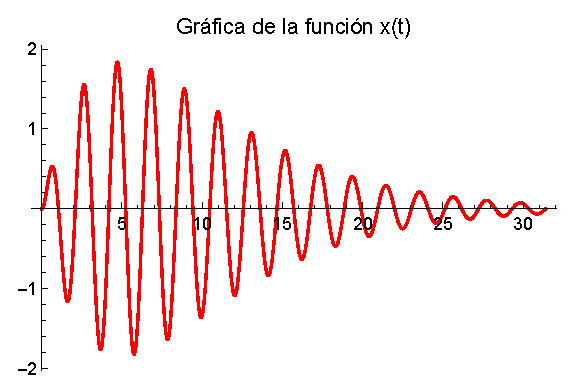
\includegraphics[scale=1]{Imagenes/Ejemplo_Resonancia_01.eps}
    % \caption{Solución de $x(t)$ vs $t$}
\end{figure}
\end{frame}
\begin{frame}
\frametitle{De la solución}
Vemos que hay un intervalo en donde se presenta un incremento de la amplitud, se alcanza el máximo de la misma en $t = 5$, para luego ir disminuyendo conforme avanza el tiempo.
\\
\bigskip
\pause
Podemos hacer un estudio adicional para encontrar más información.
\end{frame}
\begin{frame}
\frametitle{De la solución}
Es posible determinar una curva que \enquote{envuelve} a la solución $x(t)$ , \pause para determinar la curva, podemos ocupar los valores en cada cresta de $x(t)$, de tal forma que si tomamos el valor absoluto, tendremos el doble de puntos y con ello, mejorar la aproximación de la curva.
\end{frame}
\begin{frame}[plain]
\begin{figure}[H]
    \centering
    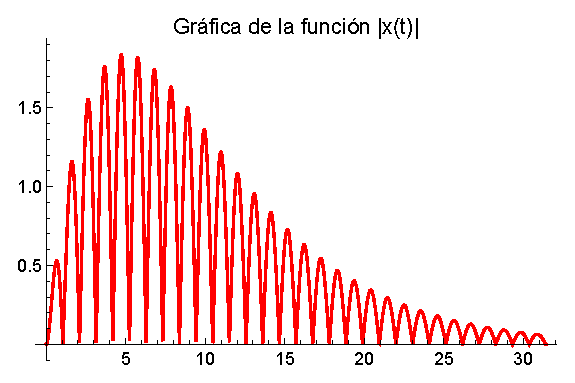
\includegraphics[scale=0.55]{Imagenes/Ejemplo_Resonancia_02.eps}
    % \caption{Al tomar el valor absoluto, se tendrán más puntos para la aproximación.}
\end{figure}
\end{frame}
\begin{frame}
\frametitle{De la solución}
Como contamos ya con un conjunto mayor de puntos, podemos ocupar su valor y realizar un análisis de mínimos cuadrados y obtener la expresión de la curva:
\end{frame}
\begin{frame}[plain]
\begin{figure}[H]
    \centering
    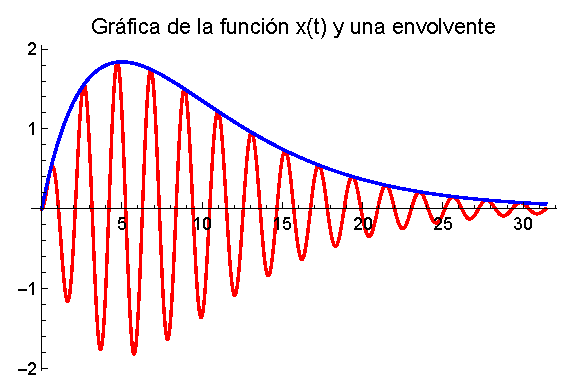
\includegraphics[scale=0.55]{Imagenes/Ejemplo_Resonancia_03.eps}
    \caption{La curva en azul es la envolvente de $x(t)$.}
\end{figure}
\end{frame}
\begin{frame}
\frametitle{De la solución}
Al ser $x(t)$ simétrica con respecto a $y = 0$, la curva envolvente para valores negativos, tendrá un signo negativo con respecto a los valores positivos.
\end{frame}
\begin{frame}[plain]
\begin{figure}[H]
    \centering
    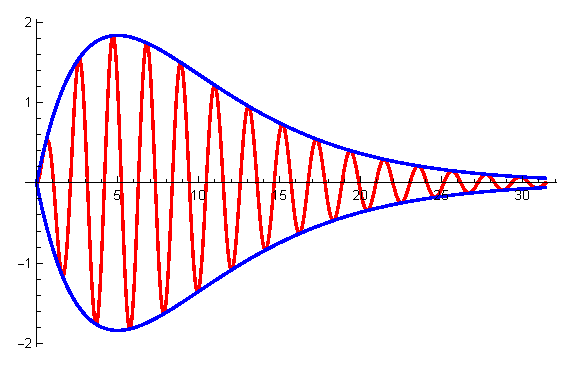
\includegraphics[scale=0.55]{Imagenes/Ejemplo_Resonancia_04.eps}
    \caption{Las curvas envolventes de $x(t)$.}
\end{figure}
\end{frame}
\begin{frame}
\frametitle{De la solución}
Al realizar el respectivo procedimiento de análisis de los datos con mínimos cuadrados, se obtiene la expresión para la curva que \enquote{envuelve} a la gráfica del desplazamiento de la masa, que en este caso resulta ser: $c = t \, \exp(-t/5)$.
\end{frame}
\begin{frame}[plain]
\begin{figure}[H]
    \centering
    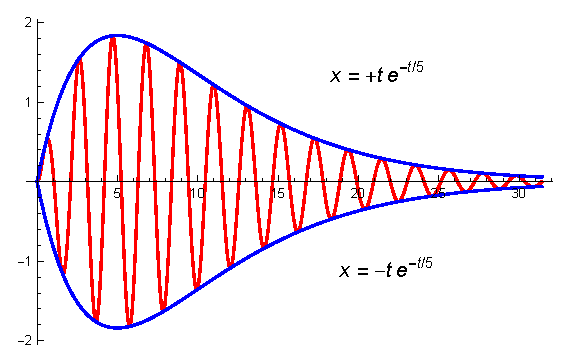
\includegraphics[scale=0.55]{Imagenes/Ejemplo_Resonancia_05.eps}
    % \caption{Las curvas envolventes de $x(t)$ como función de $t$.}
\end{figure}
\end{frame}
% \section{Transformada de Fourier.}

% \subsection{Definición.}

% Se define la transformada de Fourier como:
% \begin{align}
% F \big[ f(x); x \to \xi \big] = \dfrac{1}{\sqrt{2 \, \pi}} \scaleint{5ex}_{\bs -\infty}^{+\infty} f(x) \, \exp(i \, \xi \, x) \dd{x}
% \label{eq:ecuacion_01_12}
% \end{align}

% Mientras que la transformada inversa de Fourier se define de la siguiente manera:
% \begin{align}
% f(x) = F^{-1} \big[ F(\xi) \big] = \dfrac{1}{\sqrt{2 \, \pi}} \int_{-\infty}^{+\infty} F(\xi) \, \exp(-i \, \xi \, x) \dd{\xi}
% \label{eq:ecuacion_01_13}
% \end{align}
% en un punto continuo de $f(x)$.

% Recuerden que el detalle de las propiedades de la Transformada de Fourier se indican en las notas de trabajo, por lo que esperamos que las hayan revisado de manera oportuna.

% \subsection{Ejercicios con la Transformada de Fourier.}

% \subsection*{Primer ejercicio.}

% Evalúa la transformada de Fourier de:
% \begin{align*}
% f(x) = \begin{cases}
% x, & \abs{x} < a \\
% 0, & \abs{x} > a
% \end{cases}
% \end{align*}

% Ocupamos la definición de la transformada de Fourier, que se indica en la ec. (\ref{eq:ecuacion_01_12}), así que:
% \begin{align*}
% F \big[ f(x); x \to \xi \big] = \dfrac{1}{\sqrt{2 \, \pi}} \scaleint{5ex}_{\bs -a}^{a} x \, \exp(i \, \xi \, x) \dd{x}
% \end{align*}

% Resolvemos la integral por partes\footnote{Para abreviar el material de trabajo, se presentan los resultados, pero pueden realizar a mano todo el trabajo y corroborar que lo que mostramos es correcto.}, y obtenemos lo siguiente:
% \begin{align*}
% &= \dfrac{1}{\sqrt{2 \, \pi}} \left\{ \bigg[ x \, \dfrac{\exp(i \, \xi \, x)}{i \, \xi} \bigg] \bigg\vert_{-a}^{a} - \dfrac{1}{i \, \xi} \scaleint{5ex}_{\bs -a}^{a} \exp(i \xi \, x) \dd{x} \right\} \\[1em] 
% &= \dfrac{1}{\sqrt{2 \, \pi}} \bigg[ \dfrac{a \, e^{i \xi a} + a \, e^{-i \xi a}}{i \, \xi} + \dfrac{1}{\xi^{2}} \left( e^{i a \xi} - e^{-i a \xi} \right) \bigg] =
% \end{align*}

% Ocupando las identidades de Euler conocidas, en donde se relacionan las funciones trigonométricas, con la función exponencial, se tiene que:

% \begin{align*}
% &= \dfrac{1}{\sqrt{2 \, \pi}} \bigg[ \dfrac{2 \, a \, \cos a \xi}{i \, \xi} + \dfrac{2 \, i \, \sin a \xi}{\xi^{2}} \bigg] = \\[1em] 
% &= \sqrt{\dfrac{2}{\pi}} \, i \, \bigg[ \dfrac{\sin a \xi - a \, \xi \, \cos a \, \xi}{\xi^{2}} \bigg]
% \end{align*}

% \subsection*{Segundo ejercicio.}

% Calcula la transformada de Fourier de:
% \begin{align*}
% f(x) = \exp(-a \, \abs{x}), \hspace{1cm} a > 0
% \end{align*}

% Ocupamos nuevamente la definición de la TF, por lo que:
% \begin{align*}
% F \big[ f(x); x \to \xi \big] {=} \dfrac{1}{\sqrt{2 \pi}} \scaleint{5ex}_{\bs -\infty}^{+\infty} \exp(-a \abs{x}) \, \exp(i \xi x) \dd{x}
% \end{align*}
% Para resolver la integral, primero \enquote{separamos} en el dominio el integrando:
% \begin{align*}
% = \dfrac{1}{\sqrt{2 \pi}} \bigg[ \scaleint{5ex}_{\bs -\infty}^{0} e^{ a  x} \, e^{i \xi x} \dd{x} + \scaleint{5ex}_{\bs 0}^{\infty} e^{ -a  x} \, e^{i \xi x} \dd{x} \bigg] =
% \end{align*}

% Cada integral se resuelve directamente y se evalúa en los límites de integración, notemos que al tener en el integrado el producto de funciones exponenciales, ocupamos las propiedades de la misma, por lo que se simplifica la expresión y el cálculo de la integral es a la vez, más sencillo. Se obtiene entonces:
% \begin{align*}
% &= \dfrac{1}{\sqrt{2 \pi}} \bigg[ \dfrac{1}{a + i \, \xi} + \dfrac{1}{a - i \xi} \bigg] = \\[0.5em] 
% &= \sqrt{\dfrac{2}{\pi}} \, \dfrac{a}{a^{2} + \xi^{2}}
% \end{align*}

% %REf. Zill Cap. 7.4 Transformada de Fourier Ejemplo 2
% \section{Ecuación de calor.}
% \subsection{Temperatura en una placa semiinfinita.}


% La temperatura constante de una placa semiinfinita está dada por la siguiente ecuación diferencial, condiciones iniciales y de frontera:
% \begin{align*}
% &\pdv[2]{u}{x} + \pdv[2]{u}{y} = 0 \hspace{1cm} 0 < x < \pi, \hspace{0.3cm} y > 0 \\[0.5cm]
% &u(0, y) = 0 \hspace{1cm} u(\pi, y) = e^{-y} \hspace{0.3cm} y > 0 \\[0.5cm]
% &\pdv{u}{y} \eval_{y=0} = 0 \hspace{1cm} 0 < x < \pi
% \end{align*}

% El problema a resolver en este ejercicio es: \textbf{Encuentra el valor de temperatura de $u(x,y)$}.

% \begin{figure}[H]
%     \centering
%     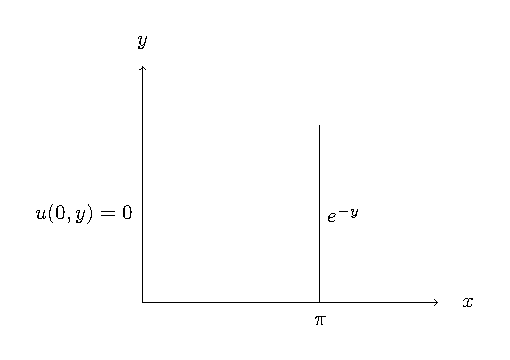
\includegraphics[scale=1.3]{Imagenes/Transformada_Fourier_Placa_Ejemplo.eps}
%     \caption{Placa semiinfinita con las condiciones iniciales que determina el problema.}
% \end{figure}

% El dominio de la variable y la condición prescrita en $y = 0$, indican que se puede aplicar la transformada coseno de Fourier al problema, definimos así:
% \begin{align*}
% F_{c} \big[u(x,y)\big] = \scaleint{5ex}_{\bs 0}^{\infty} u(x, y) \, \cos \alpha \, y \dd{y} = U(x, \alpha)
% \end{align*}


% Como la transformada coseno de Fourier de la derivada de una función es:
% \begin{align*}
% F_{c} \big[\stilde{y}(x)] = - \alpha^{2} \, F[\alpha] - \ptilde{f} (0)
% \end{align*}
% se tiene que:
% \begin{align*}
% F_{c} \left[\pdv[2]{u}{x} \right] + F_{c} \left[\pdv[2]{u}{y} \right] = F_{c} [0]
% \end{align*}
% Por lo tanto:
% \begin{align*}
% \dv[2]{U}{x} - \alpha^{2} \, &U(x, \alpha) - u_{y} (x, 0) = 0 \\[1em]
% &\Rightarrow \hspace{0.3cm} \dv[2]{U}{x} - \alpha^{2} \, U = 0
% \end{align*}
% Recordemos que $(\pdv*{u}{y})\eval_{y=0} = 0$, la EDO2H es una ecuación que ya sabemos resolver, se muestra el resultado a continuación.
% \\[0.5em]
% Puesto que el dominio de $x$ es un intervalo finito, es preferible escribir la solución a la EDO como:
% \begin{align}
% U(x, \alpha) = c_{1} \, \cosh (\alpha \, x) + c_{2} \, \sinh (\alpha \, x)
% \label{eq:ecuacion_016}
% \end{align}

% Ahora bien, las transformadas de Fourier en los puntos $x = 0$ y $x = \pi$, son:
% \begin{align*}
% F_{c} \big[ u(0, y)\big] &= F_{c} [0] \\[0.5em]
% F_{c} \big[ u(\pi, y)\big] &= F_{c} \big[ e^{-y} \big]
% \end{align*}
% y son equivalentes a:
% \begin{align*}
% U(0, \alpha) &= 0 \\[0.5em]
% U(\pi, \alpha) &= \dfrac{1}{1 +  \alpha^{2}}
% \end{align*}
% respectivamente.

% Cuando se aplican estas últimas condiciones, en la solución ec. (\ref{eq:ecuacion_016}) nos devuelve el valor de los coeficientes:
% \begin{align*}
% c_{1} &= 0 \\[0.5em]
% c_{2} &= \dfrac{1}{(1 + \alpha^{2}) \, \sinh \alpha \pi}
% \end{align*}
% Por lo tanto, la transformada coseno de Fourier es:
% \begin{align*}
% U(x, \alpha) = \dfrac{\sinh \alpha \, x}{(1 + \alpha^{2}) \, \sinh \alpha \pi}
% \end{align*}

% De modo que al ocupar la transformada coseno inversa de Fourier, tenemos que:
% \begin{align*}
% F_{c}^{-1} \big[F(\alpha)\big] = \dfrac{2}{\pi} \scaleint{5ex}_{\bs 0}^{\infty} F[\alpha] \, \cos \alpha \, x \dd{x}
% \end{align*}

% Para obtener el siguiente resultado que nos determina la solución $u(x,y)$ en los puntos dentro de la placa semiinfinita:
% \begin{align*}
% u(x, y) = \dfrac{2}{\pi} \scaleint{6ex}_{\bs 0}^{\infty} \dfrac{\sinh \alpha \, x}{(1 + \alpha^{2}) \, \sinh \alpha \pi} \, \cos \alpha \, x \dd{x}
% \end{align*}
% La solución obtenida se le conoce como \emph{solución fundamental}.

\end{document}